%\documentclass[slidestop]{beamer}
\documentclass[slidestop,uncompress,mathserif,final]{beamer}

% Import packages %
\usepackage{color, graphicx}
\usepackage[draft]{fixme}
\usepackage[utf8]{inputenc}


% Beamer theme configuration %
%\usetheme{Copenhagen} 
%\usetheme{Berlin} 
%\usetheme{Berkeley} 
\usetheme{Singapore} 
%\usetheme{Warsaw} 
%\usetheme{umbc1} 
%\usetheme{umbc2} 
%\usetheme{umbc3} 
%\usetheme{umbc4} 
%\usefonttheme{structuresmallcapsserif}
%\useoutertheme[subsection=false,footline=authorinstitute]{smoothbars}
%\setbeamertemplate{navigation symbols}{}


% Util commands %
\newcommand{\pgl}[0]{Peter Gorm Larsen} 
\newcommand{\mail}[1]{{\small \texttt{#1}}}
\newcommand{\yellow}[1]{{\color{yellow} #1}}
\newcommand{\blue}[1]{{\color{blue} #1}}
\newcommand{\red}[1]{{\color{red} #1}}
\newcommand{\green}[1]{{\color{green} #1}}
\newcommand{\fixin}[1]{\fixme[inline]{\texttt{#1}}} 
\newcommand{\fixfo}[1]{\fixme[footnote]{\texttt{#1}}} 
\newcommand{\fixma}[1]{\fixme[margin]{\texttt{#1}}} 
\newcommand{\from}[1]{%
\noindent%
\begin{flushright}%
    \emph{\footnotesize #1}%
\end{flushright}%
} 


% title slide %
\title[Bootstrapping in Overture]{Bootstrapping tools for VDM in Overture}


\subtitle{Rodin User and Developer Workshop}

\author[K. Lausdahl, M. Ferreira]{
  Kenneth Lausdahl \\
  \mail{kenneth AT lausdahl.com} \\
  Miguel Ferreira \\
  \mail{m.ferreira AT sig.nl}
}

\institute[IHA, SIG]{
  Aarhus School of Engineering\\
  Software Improvement Group
}

\date{July ?, 2009 --- Southampton}


\begin{document} 

\begin{frame}[c]
	\titlepage
\end{frame}

\begin{frame}[c]
  \frametitle{Outline}
  \tableofcontents %[pausesections] %[current,currentsubsection]
%  \tableofcontents[current]
\end{frame}

%\section[History]{History of VDM Bootstrapping} 
%\label{sec:history}

\section{Bootstrapping}
\label{sec:bootstrapping}

\begin{frame}[c]
  \frametitle{Bootstrapping}
  \framesubtitle{Compilers}


  \begin{quotation}
	``Bootstrapping is a term used in computer science to describe the techniques involved in \textbf{writing a compiler} (\dots) in the \textbf{target programming language} which \textbf{it is intended to compile}.''
  \end{quotation}
  \from{From Wikipedia, the free encyclopedia}

  \pause
  \begin{itemize}
	\item Instantiation of the \alert{chicken and egg} problem.
  \end{itemize}
\end{frame}

\begin{frame}[t]
  \frametitle{Bootstrapping}
  \framesubtitle{How is it done?}

  \pause
  \begin{itemize}
	\item How to produce the first \alert{compiler} for a new \alert{language}?
  \end{itemize}

  \vspace{\fill}

  \pause
  \begin{block}{Niklaus Wirth --- the first Pascal compiler}
  \begin{itemize}
	\itemsep=.5cm
	\item Used a \alert{different language}  --- first implementation was written in Fortan;
	  \pause
	\item \alert{Manually compiled} the compiler --- second implementation was written in Pascal and hand compiled.
  \end{itemize}
  \end{block}
\end{frame}

\section[VDMTools]{History of VDMTools Bootstrapping --- \pgl~\cite{Larsen01}} 
\label{sec:vdmtools}

\begin{frame}[c]
  \frametitle{Outline}
  \tableofcontents[current]
\end{frame}


\begin{frame}[c]
  \frametitle{Architecture}
  \framesubtitle{Overview}
  %\framesubtitle{\emph{\pgl~\cite{Larsen01}}}

  \begin{center}
    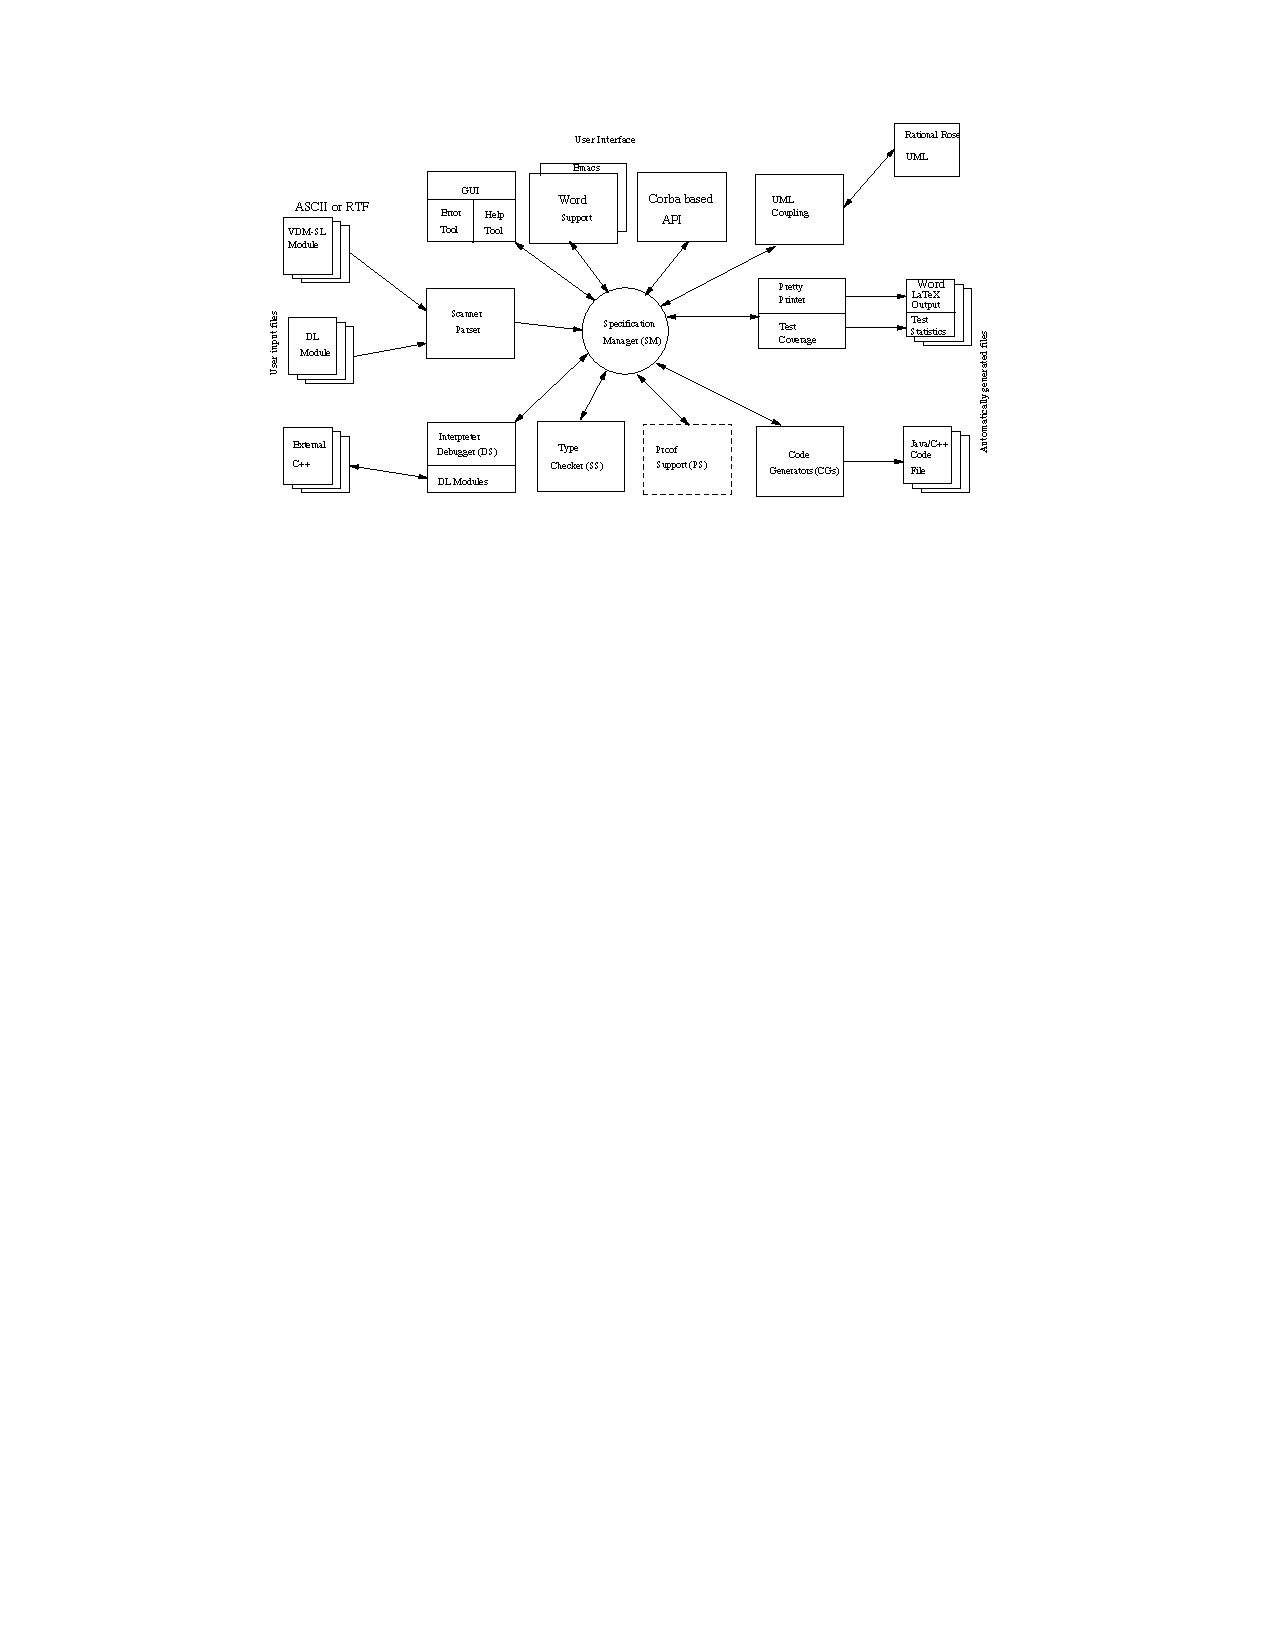
\includegraphics[width=\textwidth]{images/vdmtools_arch.pdf}
  \end{center}
%  \from{\pgl \cite{Larsen01}}
\end{frame}

\note{
4 main groups:
\begin{itemize}
  \item front end: parser, uml link
  \item validation tools: type checker, interpreter, debugger, proof support
  \item back end: code generator, pretty printer, uml link
  \item user and application interface: gui, editor connection, corba
\end{itemize}
}

\begin{frame}[c]
  \frametitle{Architecture}
  %\framesubtitle{Conventional development --- \emph{\pgl~\cite{Larsen01}}}
  \framesubtitle{Conventional development}

  \begin{center}
    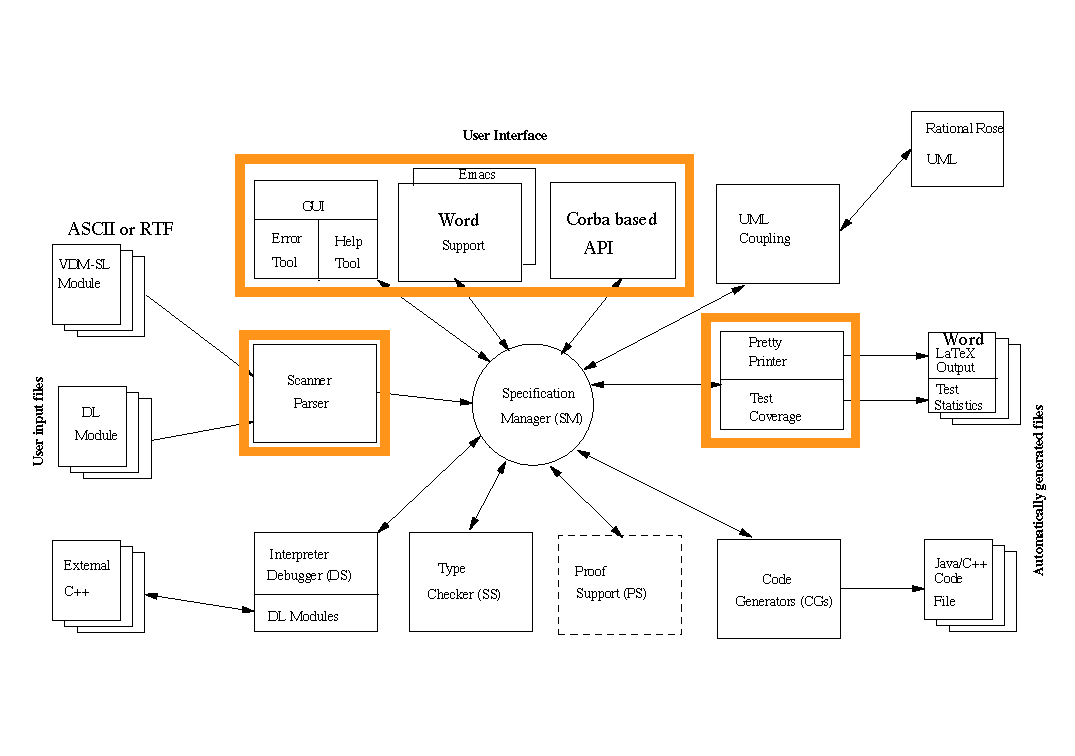
\includegraphics[width=\textwidth]{images/vdmtools_arch_conv_dev.pdf}
  \end{center}
\end{frame}

\begin{frame}[c]
  \frametitle{Architecture}
  %\framesubtitle{Formally specified --- \emph{\pgl~\cite{Larsen01}}}
  \framesubtitle{Formally specified}

  \begin{center}
    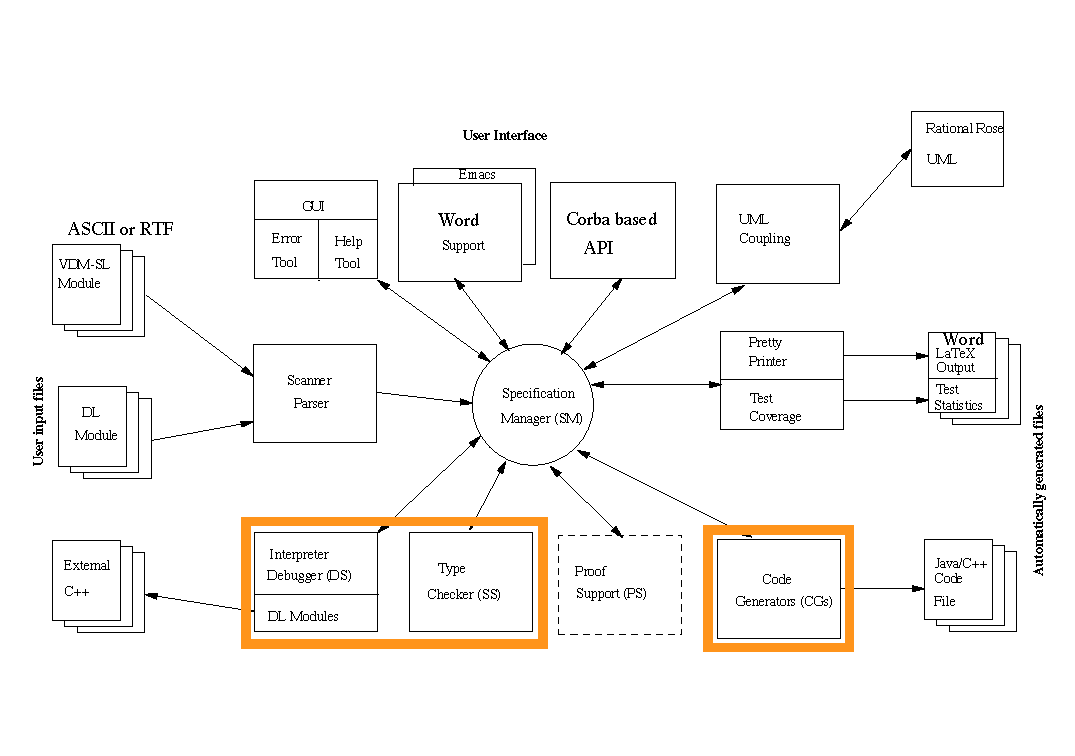
\includegraphics[width=\textwidth]{images/vdmtools_arch_spec.pdf}
  \end{center}
\end{frame}

\begin{frame}[c]
  \frametitle{Architecture}
  %\framesubtitle{Generated code --- \emph{\pgl~\cite{Larsen01}}}
  \framesubtitle{Generated code}

  \begin{center}
    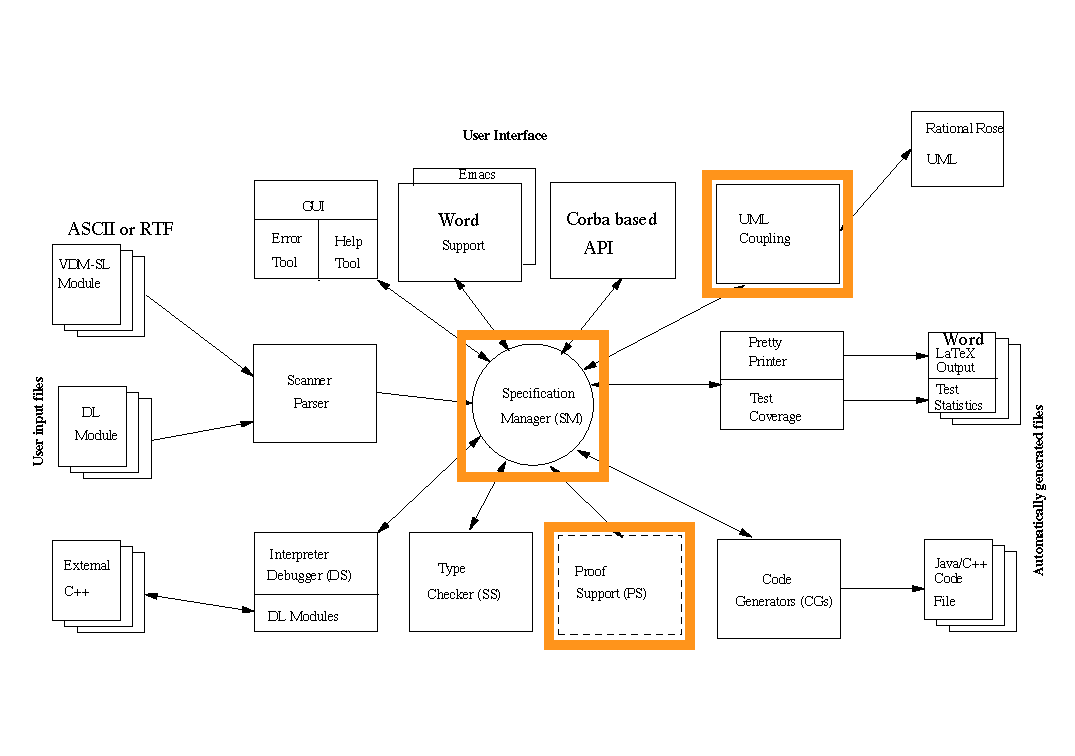
\includegraphics[width=\textwidth]{images/vdmtools_arch_cg.pdf}
  \end{center}
\end{frame}


\begin{frame}[c]
  \frametitle{Bootstrapping}
  %\framesubtitle{Test and improvement --- \emph{\pgl~\cite{Larsen01}}}
  \framesubtitle{Test and improvement}
 
  \begin{center}
    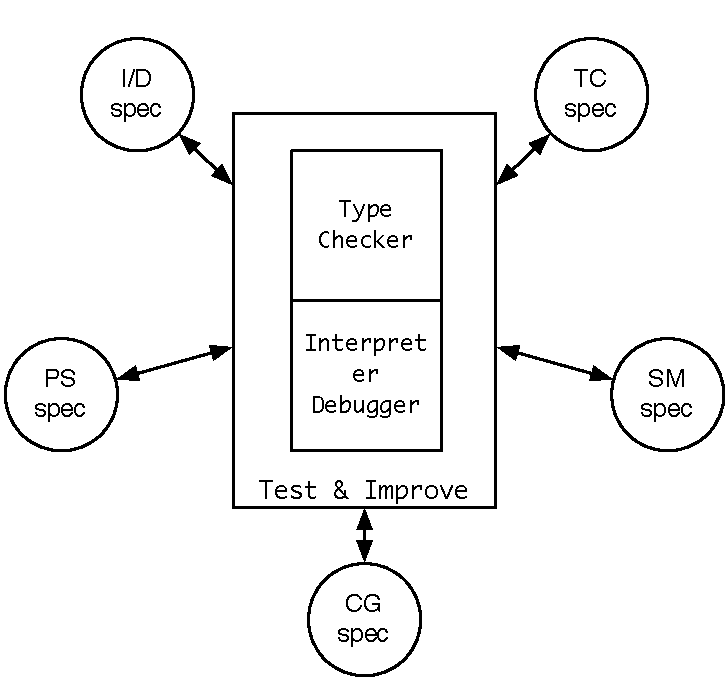
\includegraphics[width=.6\textwidth]{images/test_improve.pdf}
  \end{center}
\end{frame}

\begin{frame}[c]
  \frametitle{Bootstrapping}
  %\framesubtitle{Tool generation --- \emph{\pgl~\cite{Larsen01}}}
  \framesubtitle{Tool generation}

  \begin{center}
    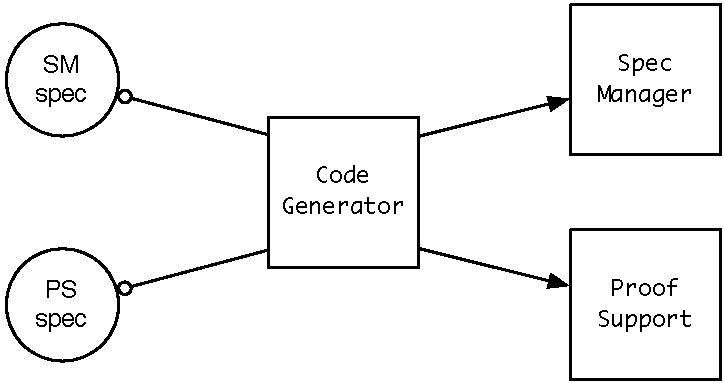
\includegraphics[width=.7\textwidth]{images/code_gen.pdf}
  \end{center}
\end{frame}

\begin{frame}[c]
  \frametitle{Bootstrapping}
  %\framesubtitle{Tool generation --- \emph{\pgl~\cite{Larsen01}}}
  \framesubtitle{Tool generation}
 
  \begin{center}
    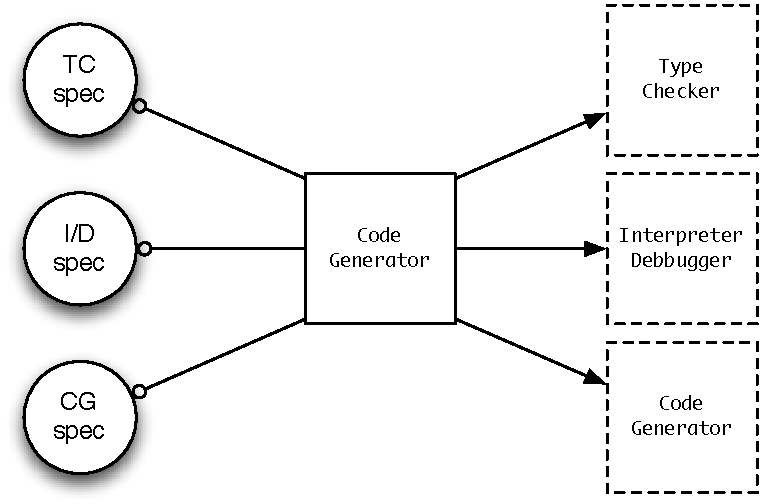
\includegraphics[width=.7\textwidth]{images/code_gen2.pdf}
  \end{center}
\end{frame}



\section[Overture]{Bootstrapping Overture Tools for VDM}
\label{sec:overture}

\begin{frame}[c]
  \frametitle{Outline}
  \tableofcontents[current]
\end{frame}

\begin{frame}[c]
  \frametitle{Architecture}
  \framesubtitle{Overview}

  \begin{center}
    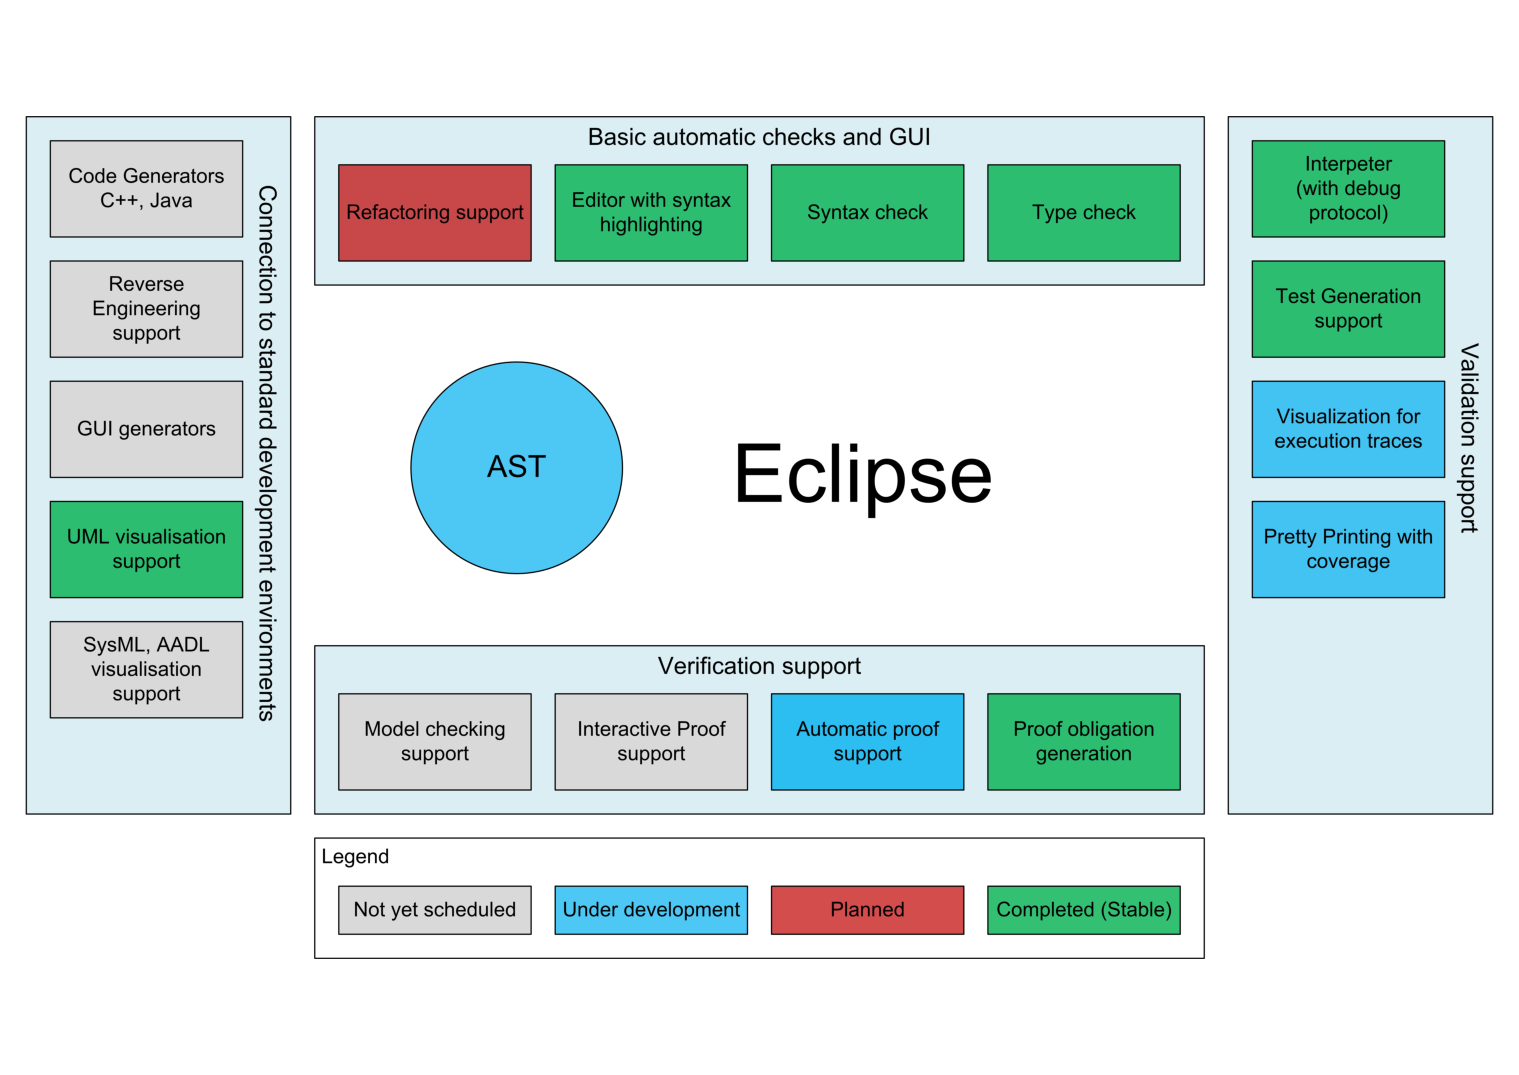
\includegraphics[width=\textwidth]{images/overture_arch.pdf}
  \end{center}
\end{frame}

\note{
\begin{itemize}
\item AST plays a key role in the arch because it is (should be) the pillar that supports all other components.
\item Objective: interoperability to achieve an integrated tool set.
\end{itemize}
}

\begin{frame}[c]
  \frametitle{Architecture}
  \framesubtitle{Conventional development}

  \begin{center}
    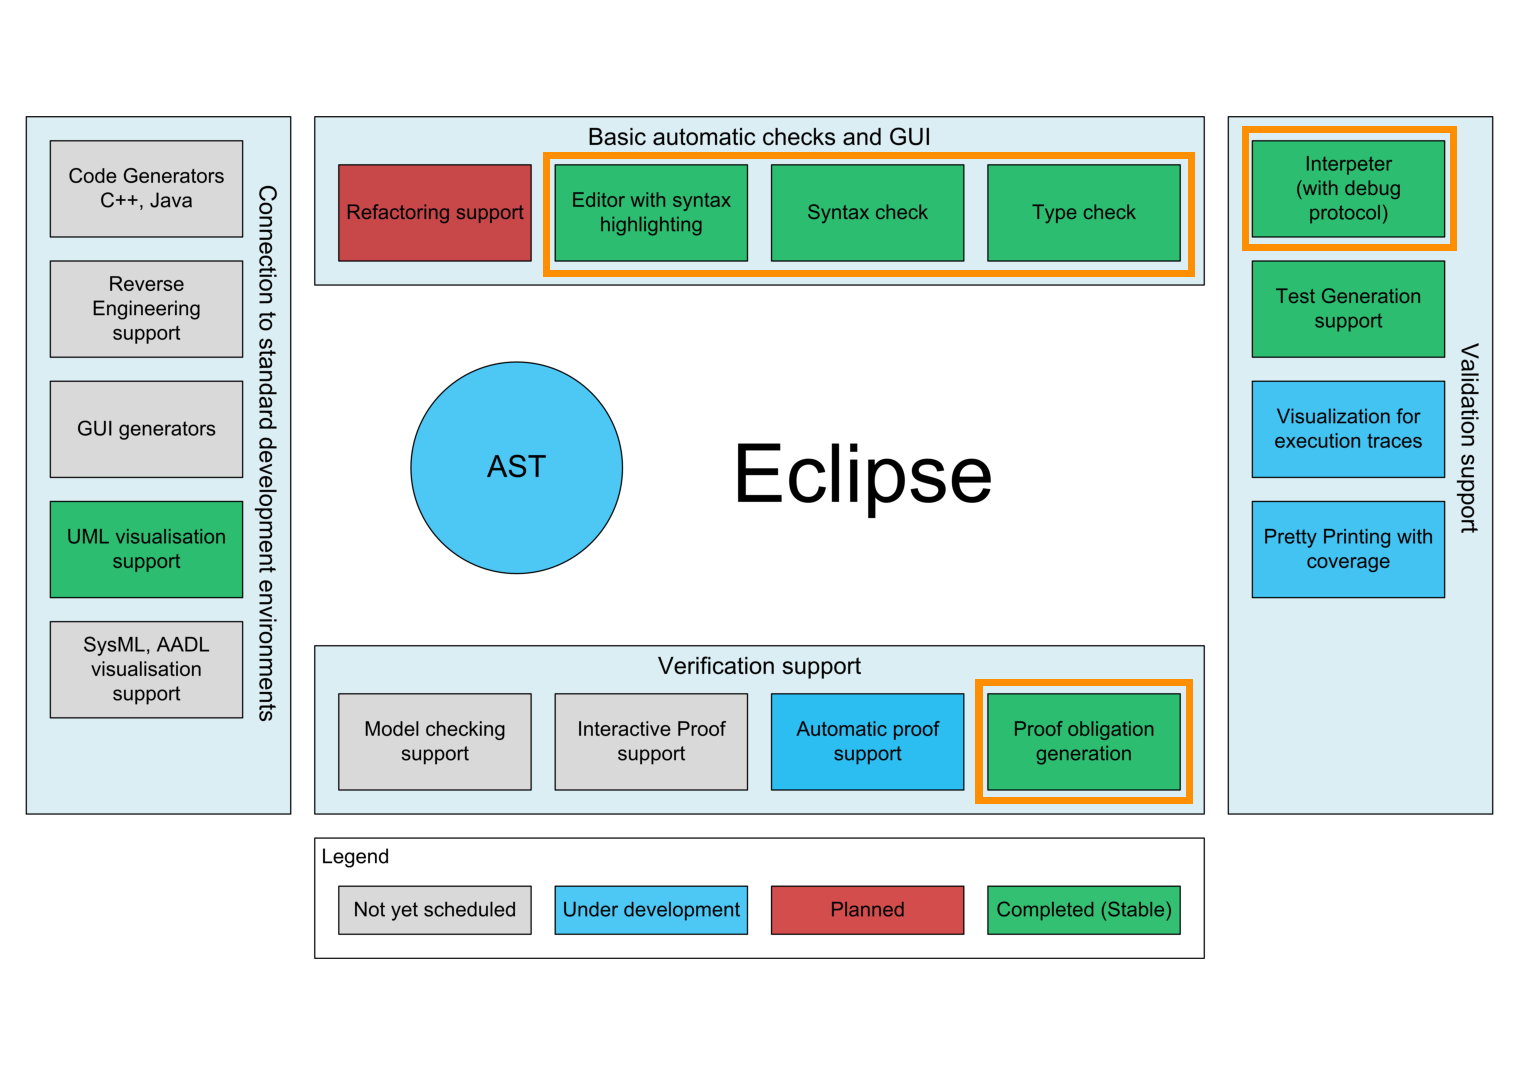
\includegraphics[width=\textwidth]{images/overture_arch_conv_dev.pdf}
  \end{center}
\end{frame}

\begin{frame}[c]
  \frametitle{Architecture}
  \framesubtitle{Formally specified}

  \begin{center}
    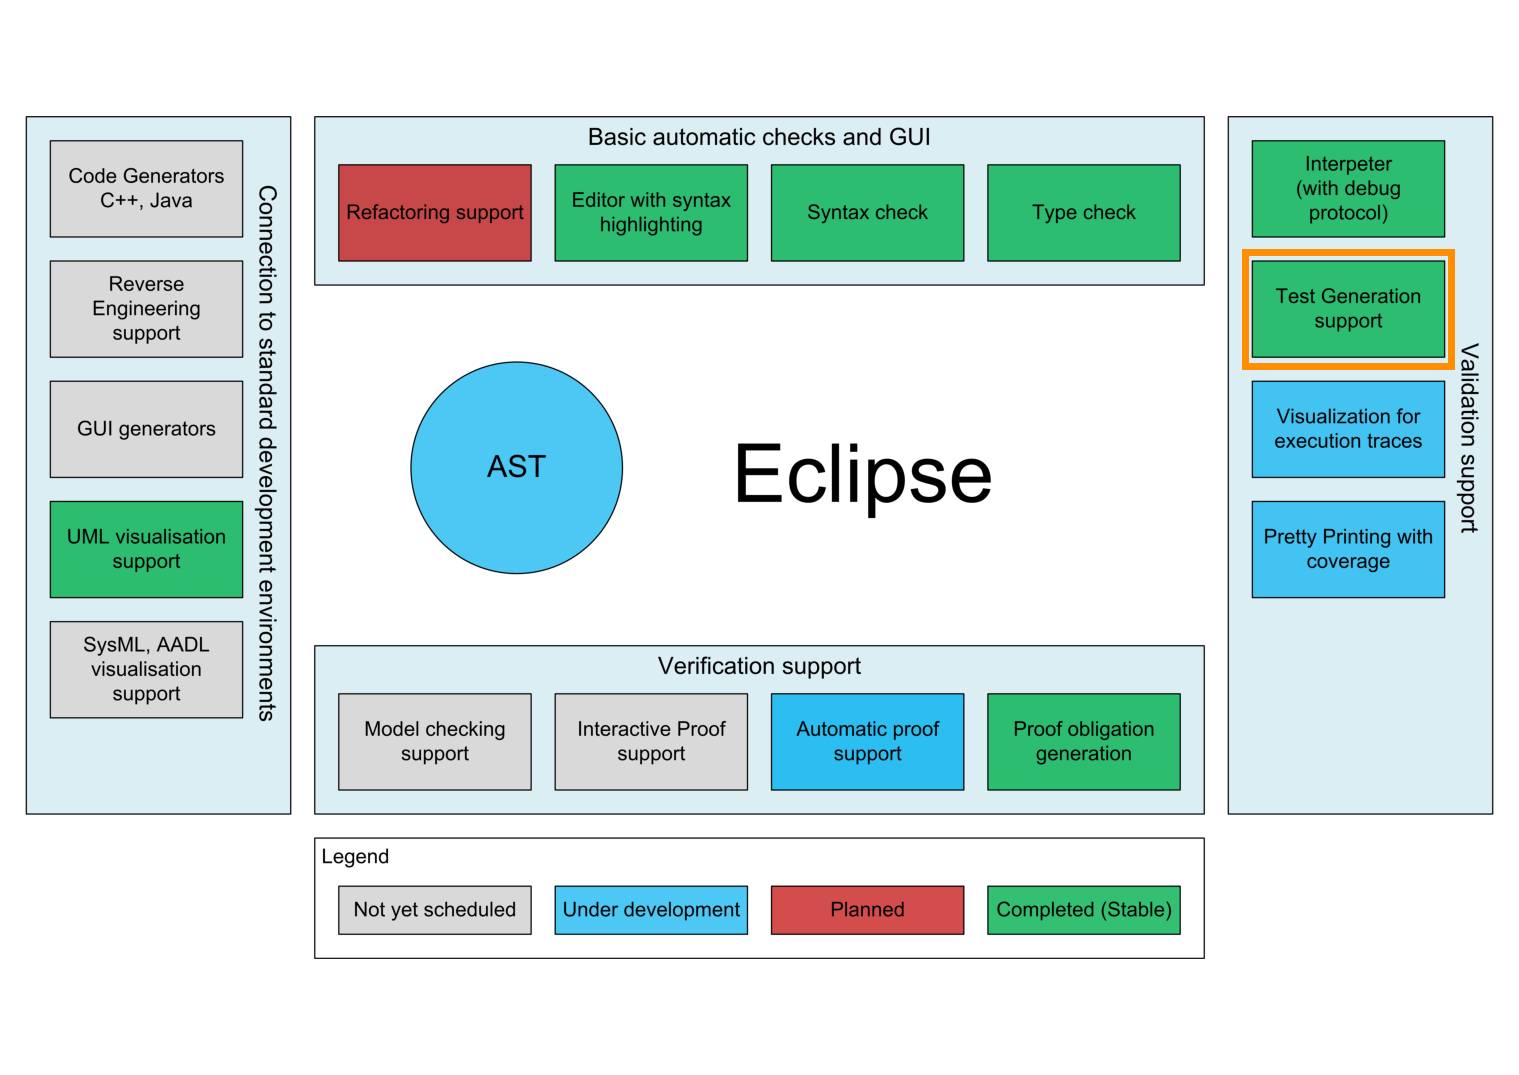
\includegraphics[width=\textwidth]{images/overture_arch_spec.pdf}
  \end{center}
\end{frame}

\begin{frame}[c]
  \frametitle{Architecture}
  \framesubtitle{Generated code}

  \begin{center}
    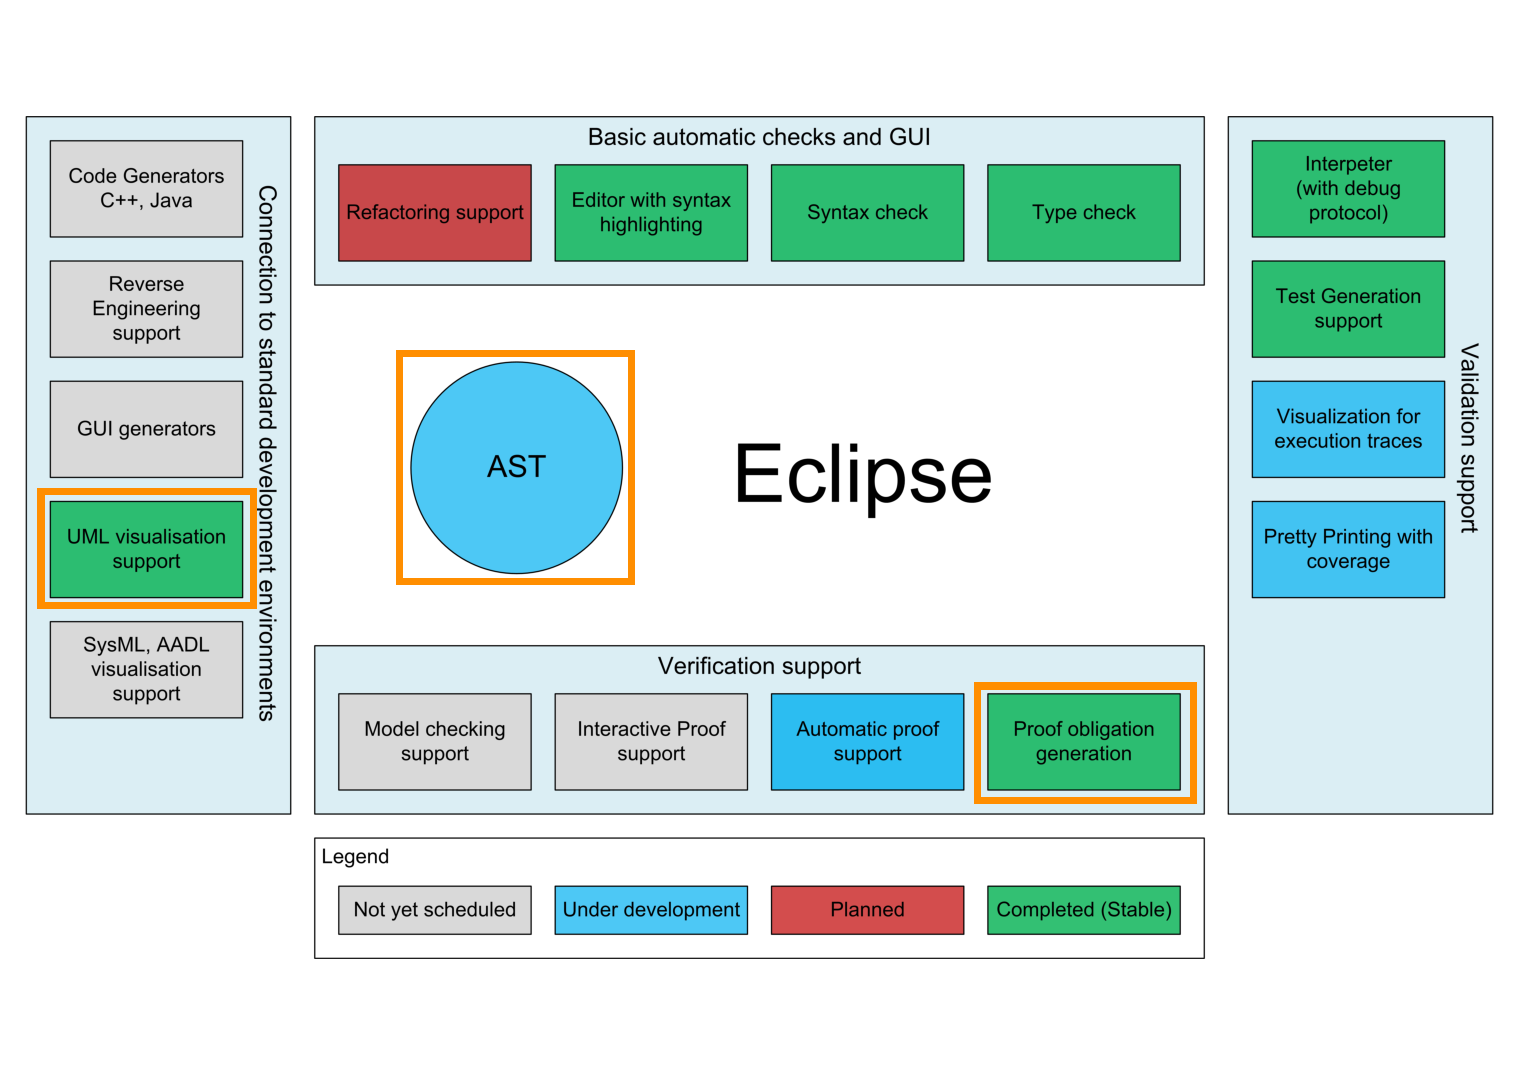
\includegraphics[width=\textwidth]{images/overture_arch_cg.pdf}
  \end{center}
\end{frame}

\begin{frame}[c]
  \frametitle{Bootstrapping}
  \framesubtitle{}


  \begin{center}
    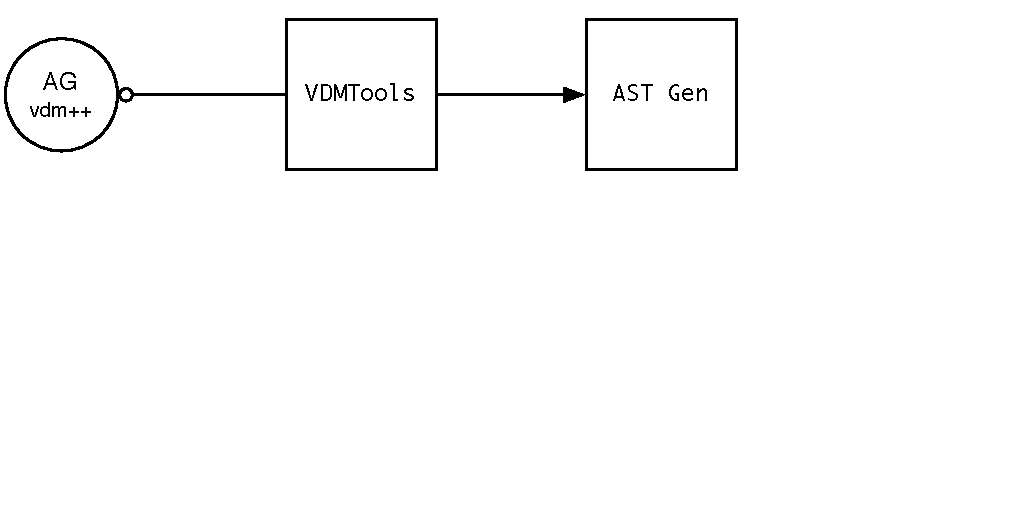
\includegraphics[width=\textwidth]{images/ast_gen_oml_ast_gen.pdf}
  \end{center}

\end{frame}

\begin{frame}[c]
  \frametitle{Bootstrapping}
  \framesubtitle{}


  \begin{center}
    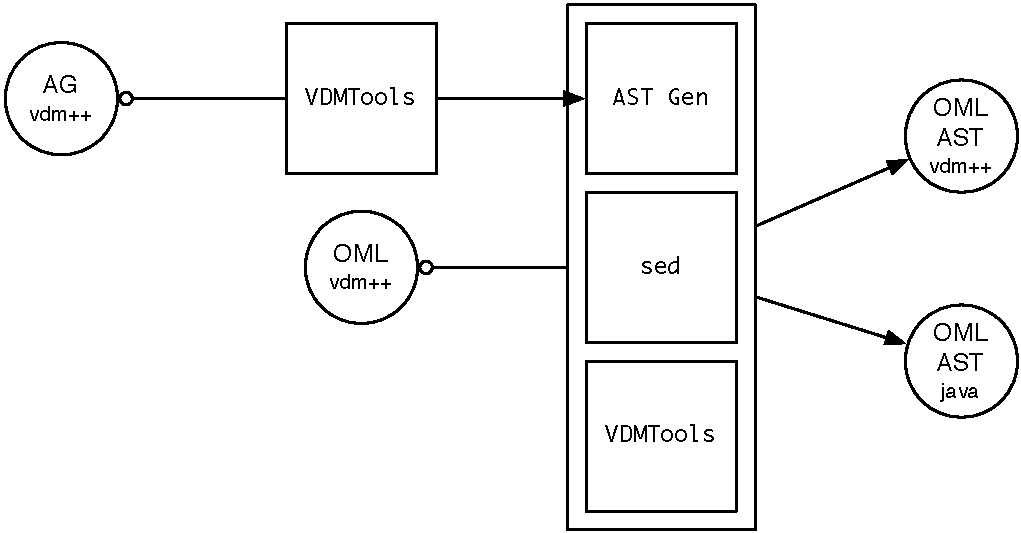
\includegraphics[width=\textwidth]{images/ast_gen_oml_ast_gen_2.pdf}
  \end{center}

\end{frame}


\note{
\begin{itemize}
  \item ASTGen plays a key role in Overture bootstrapping.

  \item It allows for AST generation from a VDM-SL spec of the language.

  \item It was used to generate both VDM++ and Java classes for the Overture Modelling Language.

  \item But can also be used to generate ASTs for other languages. Allows:
	\begin{itemize}
	  \item for agile development of language extensions
	  \item to specify other languages in VDM and have the AST in both VDM++ and Java classes
	  \item to specify translators in VDM (from which implementations can be generated) 
	\end{itemize}
\end{itemize}
}

\begin{frame}[c]
  \frametitle{Bootstrapping}
  \framesubtitle{}

  \begin{center}
    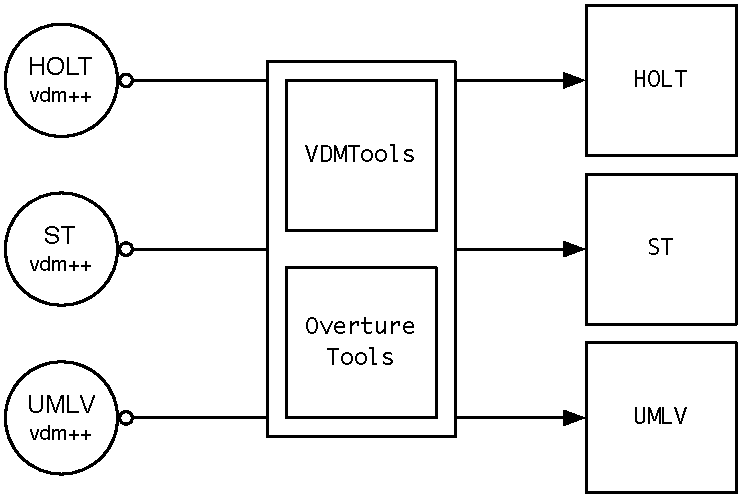
\includegraphics[width=.8\textwidth]{images/ovt_bootstrap.pdf}
  \end{center}

\end{frame}


\bibliographystyle{plain}
\bibliography{mf}

\end{document} 